\section{STATIC STRUCTURAL ANALYSIS}
\normalsize{The reflector tile assembly is a highly constrained mechanical system that wont just face high thermal flux but also is mounted on a complex frame. The heat sink is brazed on a tube that runs along the whole module with other heat sinks from other tiles brazed onto it. Some of the tiles are held using support pins welded on the \acrshort{PV}. Those pins have a limited range of motion that could potentially negatively impact the structural integrity of the tile. Structural analysis will help understand the local mechanical behavior of the tile as well as the influence of the \acrshort{BCs}.}
\subsection{Analysis of the boundary conditions influence}
\normalsize{In his 2019 analysis \cite{zhu_parametric_2019}, J. Zhu performed his \acrshort{FE} analysis using specific \acrshort{BCs} which were:
\begin{itemize}
    \item One end of the \acrshort{SS} cooling pipe fixed.
    \item The other end completely free. 
\end{itemize}
This strategy is a good approach but could be not realistic by allowing too much motion. This is why is it important to test if this modelling strategy influences the results. This \acrshort{BCs} set will be used as a reference and a series of simulations will test other \acrshort{BCs} with different numbers of degrees of freedom. This should help assess the impact of the tube and the neighboors of the studied tile on its mechanical behavior.}
\\
\break
\normalsize{\indent To perfom this analysis, first, the model used by for the thermal analyses is reused (to stay consistent with the modelling). The boundary conditions are the same as the ones from \cite{zhu_parametric_2019}.}
\\
\begin{figure}[!ht]
    \label{fig_5_14} 
    \centering
    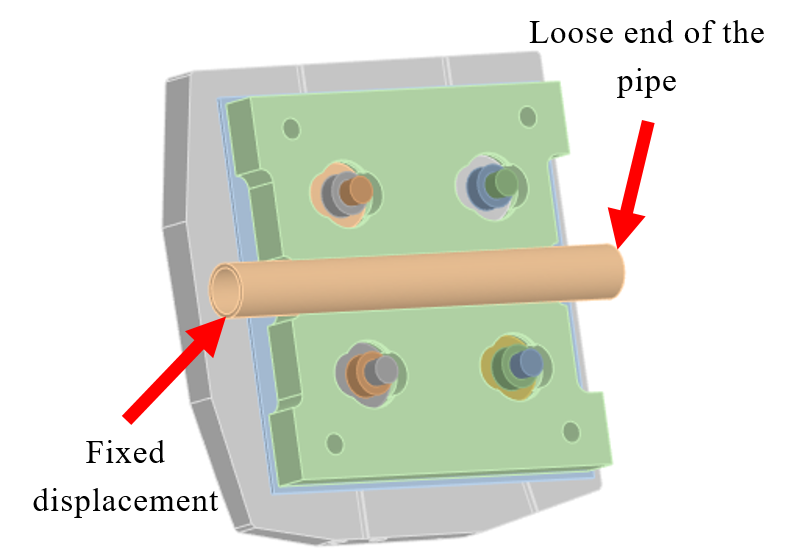
\includegraphics[width=.8\textwidth]{figures/BCStructuralConfig.png}
    \caption{\it Boundary conditions for the reference case (0).}
\end{figure}
\\
\normalsize{\indent For an accurate modelling of the tube and the heat sinks, the whole module ($H-02$) \ref{PlasmaHLonKiPModules} is cut to only feature the two supports on which the reflector tile heat sink is brazed on. The model doesn't feature the graphite/\acrshort{TZM} tiles nor the bolting system to simplifiy the calculations.}
\begin{figure}[!ht]
    \label{fig_5_15} 
    \centering
    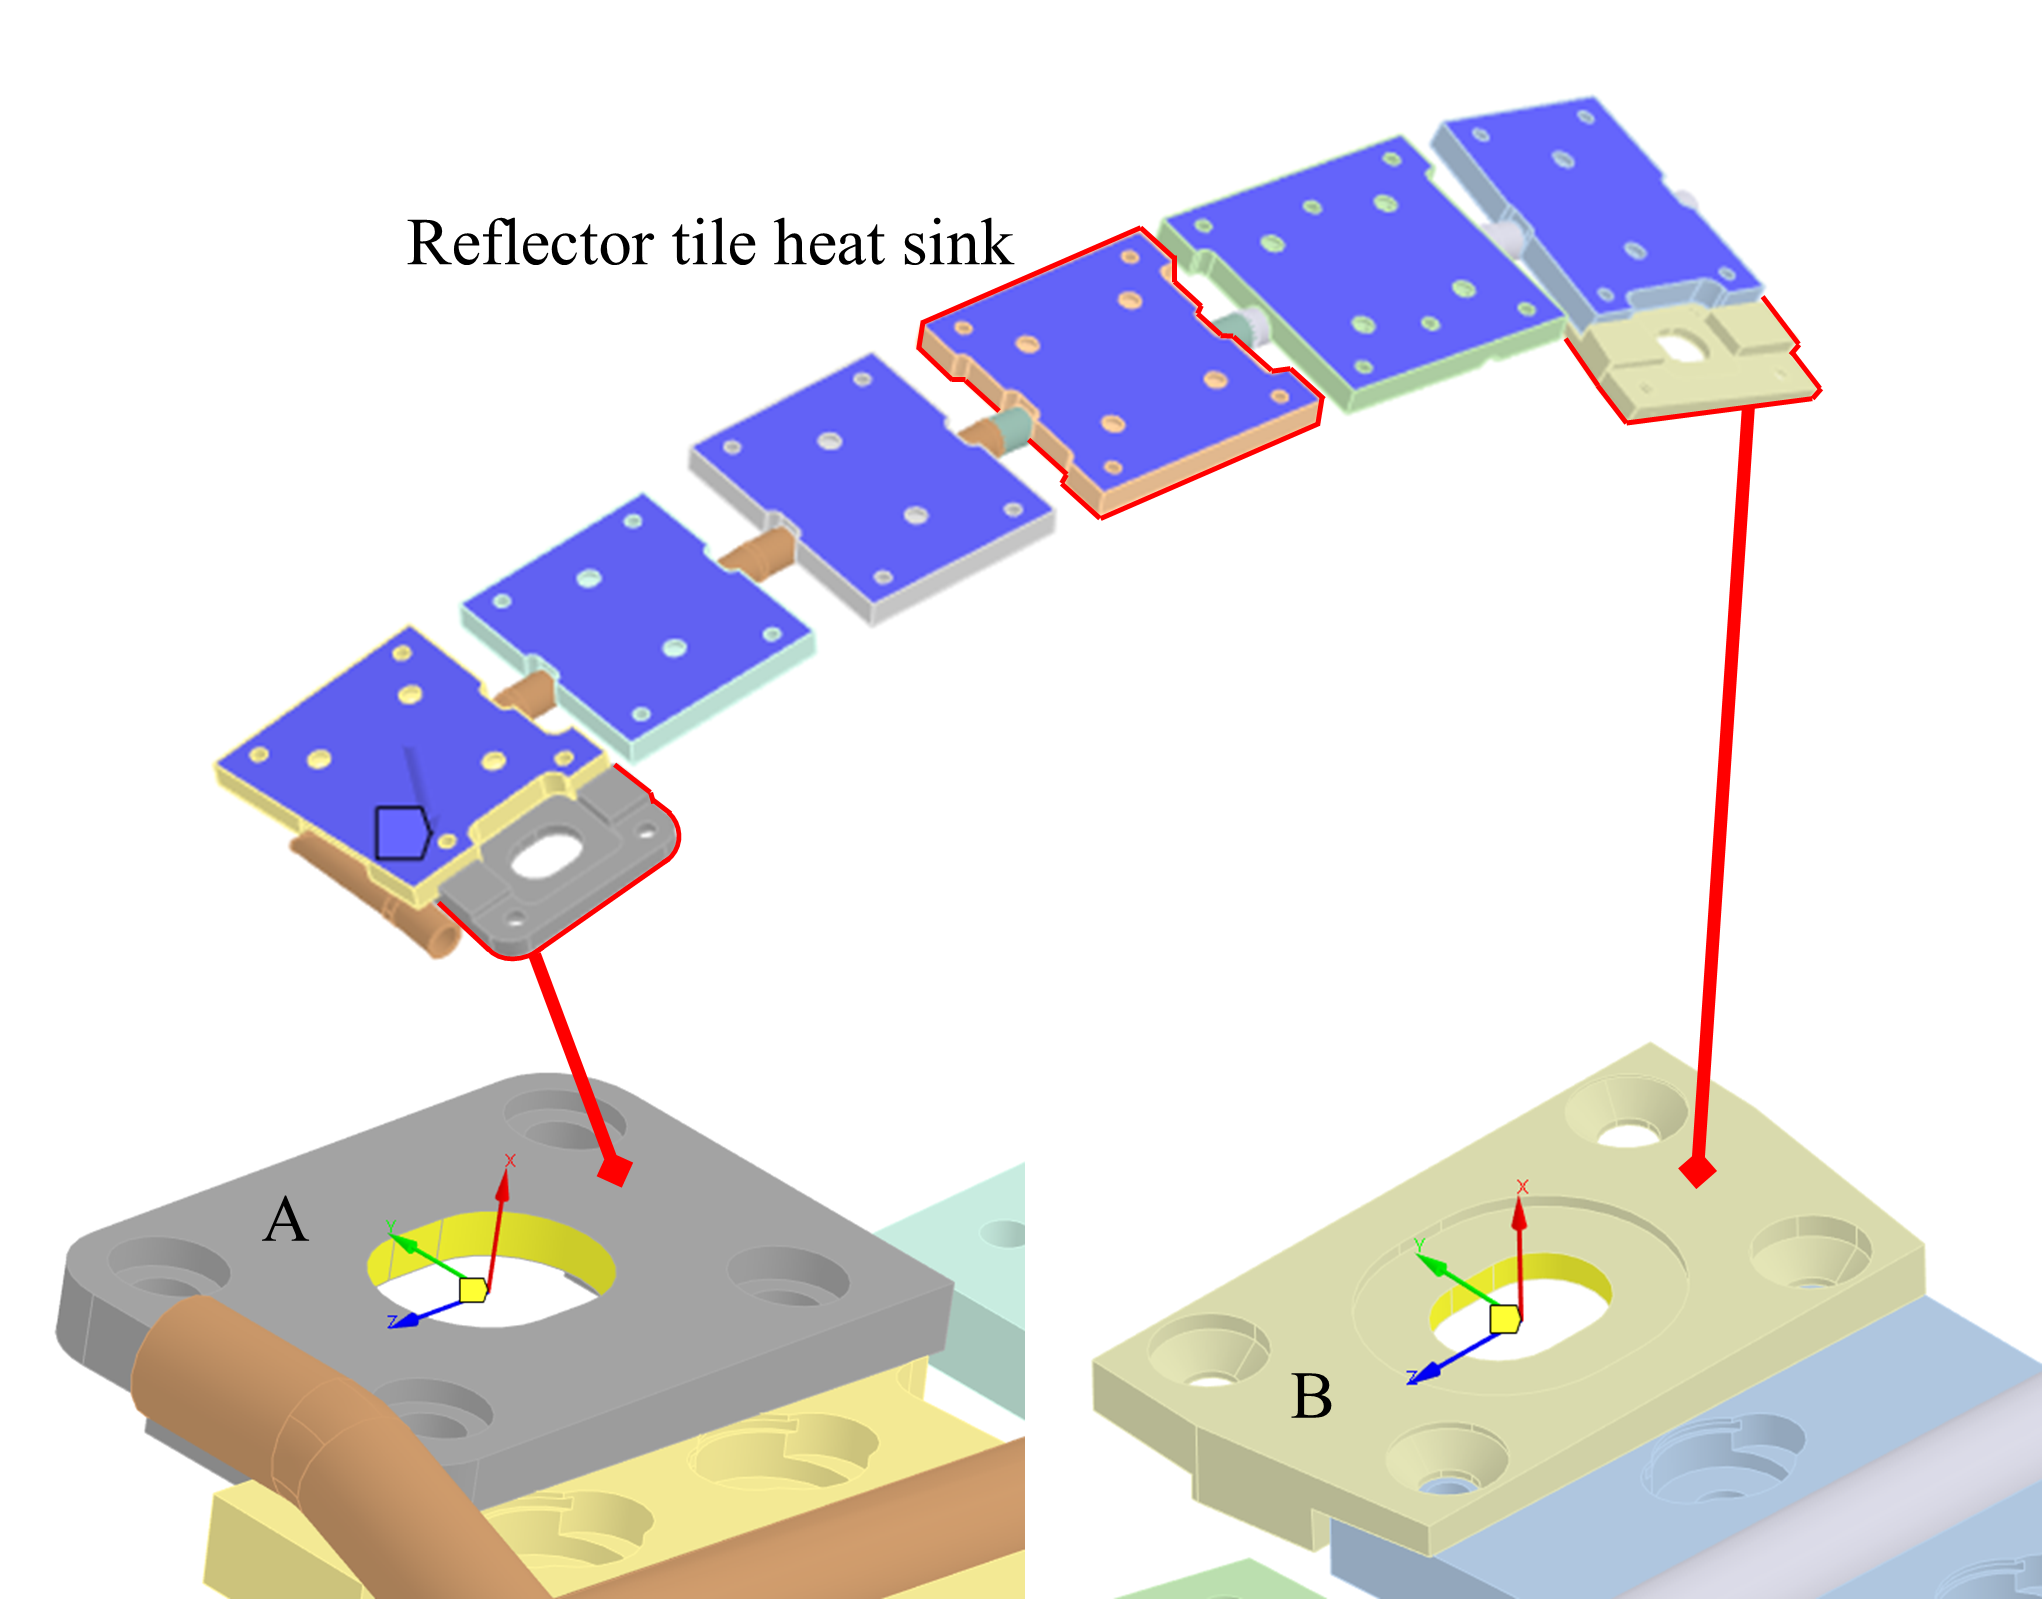
\includegraphics[width=1\textwidth]{figures/one3rdOfModule.png}
    \caption{\it View of the third of module $H-02$ with the support parts and heat sinks of adjacent tiles. A is the support that will be jointed and B is the fixed support}
\end{figure}
\\
\normalsize{\indent The supports are welded onto the \acrshort{PV} but can still move is some directions. The motions of A is controlled via a remote displacement (which works like a screw with three translational \acrshort{DoF} \{TX,TY,TZ\} and three rotational \acrshort{DoF} \{RX,RY,RZ\}) whose \acrshort{DoF} are piloted by load cases.}
\\

\begin{table*}[h!]
    \centering
    %\caption{Power conservation summary table}
    \label{table:5.5}
    \ra{1.3}
    % \begin{tabular}{@{}ccccccc@{}}
    \begin{tabular}{p{1,7cm}p{0,5cm}p{0,5cm}p{0,5cm}p{0,5cm}p{0,5cm}p{0,5cm} }
    \toprule
    $Load \ cases$ & $TX$ & $TY$ & $TZ$ & $RX$ & $RY$ & $RZ$ \\
    \cmidrule{1-7}

    1 & 0 & 0 & free & 0 & 0 & 0 \\
    \myrowcolour
    2 & 0 & 0 & free & free & 0 & free \\
    3 & 0 & 0 & free & free & free & free \\
    \myrowcolour
    4 & 0 & free & free & free & free & free \\
    5 & free & free & free & free & free & free \\

    % \midrule
\bottomrule
\end{tabular}
\caption{Table of free and fixed \acrshort{DoF} for the support A.}
\end{table*}

\normalsize{\indent The calculations were done using a coupled-field (thermal and structural) solver for practical reasons, one-way coupling would also have been perfectly adapted to this problem. The results of the analysis show different maximum displacement of the module.}
\\
\begin{figure}[!ht]
    \label{fig_5_16} 
    \centering
    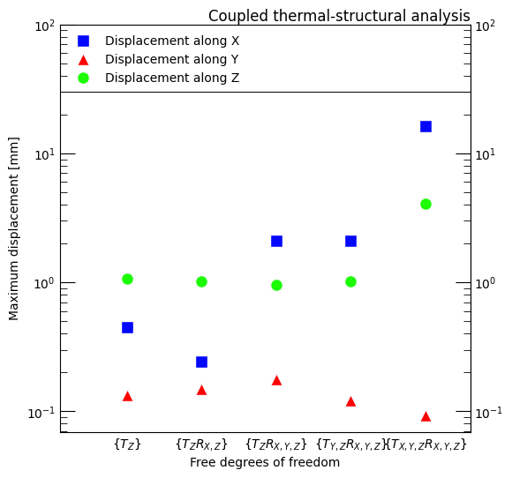
\includegraphics[width=.7\textwidth]{figures/one3rdOfModuleDisplacement.png}
    \caption{\it Maximum displacement of the module in function of freed \acrshort{DoF}.}
\end{figure}
\\
\normalsize{\indent To further assess the validitiy of the model, it is possible to compare the maximum stress of the model for each load case to the Case 0. The stress shouldn't change with respect to load case and only change because of fictitious stress concentration introduced by the mesh.}

\begin{table*}[h!]
    \centering
    %\caption{Power conservation summary table}
    \label{table:5.6}
    \ra{1.3}
    % \begin{tabular}{@{}ccccccc@{}}
    \begin{tabular}{p{1,5cm}p{1,2cm}p{1,2cm}p{1,5cm} }
    \toprule
    $\makecell{Heat \ sink \\ stress \ for \\ Case \ 0}$ & $Load case$ & $\makecell{Heat \ sink \\ max. \ stress}$ & $\makecell{Relative \\ deviation \\ to \ case \ 0}$\\
    \cmidrule{1-4}
    [\unit{Pa}] & - & [\unit{Pa}] & \% \\
    \midrule
    8,66E+08 & 1 & 7,66E+8 & 11,5 \\
    \myrowcolour
    8,66E+08 & 2 & 7,65E+8 & 11,6 \\
    8,66E+08 & 3 & 7,91E+8 & 8,6 \\
    \myrowcolour
    8,66E+08 & 4 & 8,03E+8 & 7,3 \\
    8,66E+08 & 5 & 8,85E+8 & 2,2 \\

    % \midrule
\bottomrule
\end{tabular}
\caption{Comparison of the maximum stress concentration in the heat sink.}
\end{table*}
\normalsize{\indent It is possible to conclude that the boundary conditions of Case 0 are usable as is for further structural calculations.}
\subsection{Contact status after calculations with 100 \% contact between TZM-tile and Sigraflex thermal gasket}
\normalsize{While performing the structural analysis, the contact status changed. Because the parts of the tile assembly would bend and deform due to thermal expansion, some contacts, namely the \acrshort{TZM} tile/Sigraflex contact and the Sigraflex/\acrshort{CuCrZr} heat sink contact would be broken making heat transfer via conduction impossible. The surface area would be smaller and there would not be as much heat evacuated. The 100 \% contact model thus doesn't accurately represent reality.}
\\
\begin{figure}[!ht]
    \label{fig_5_17} 
    \centering
    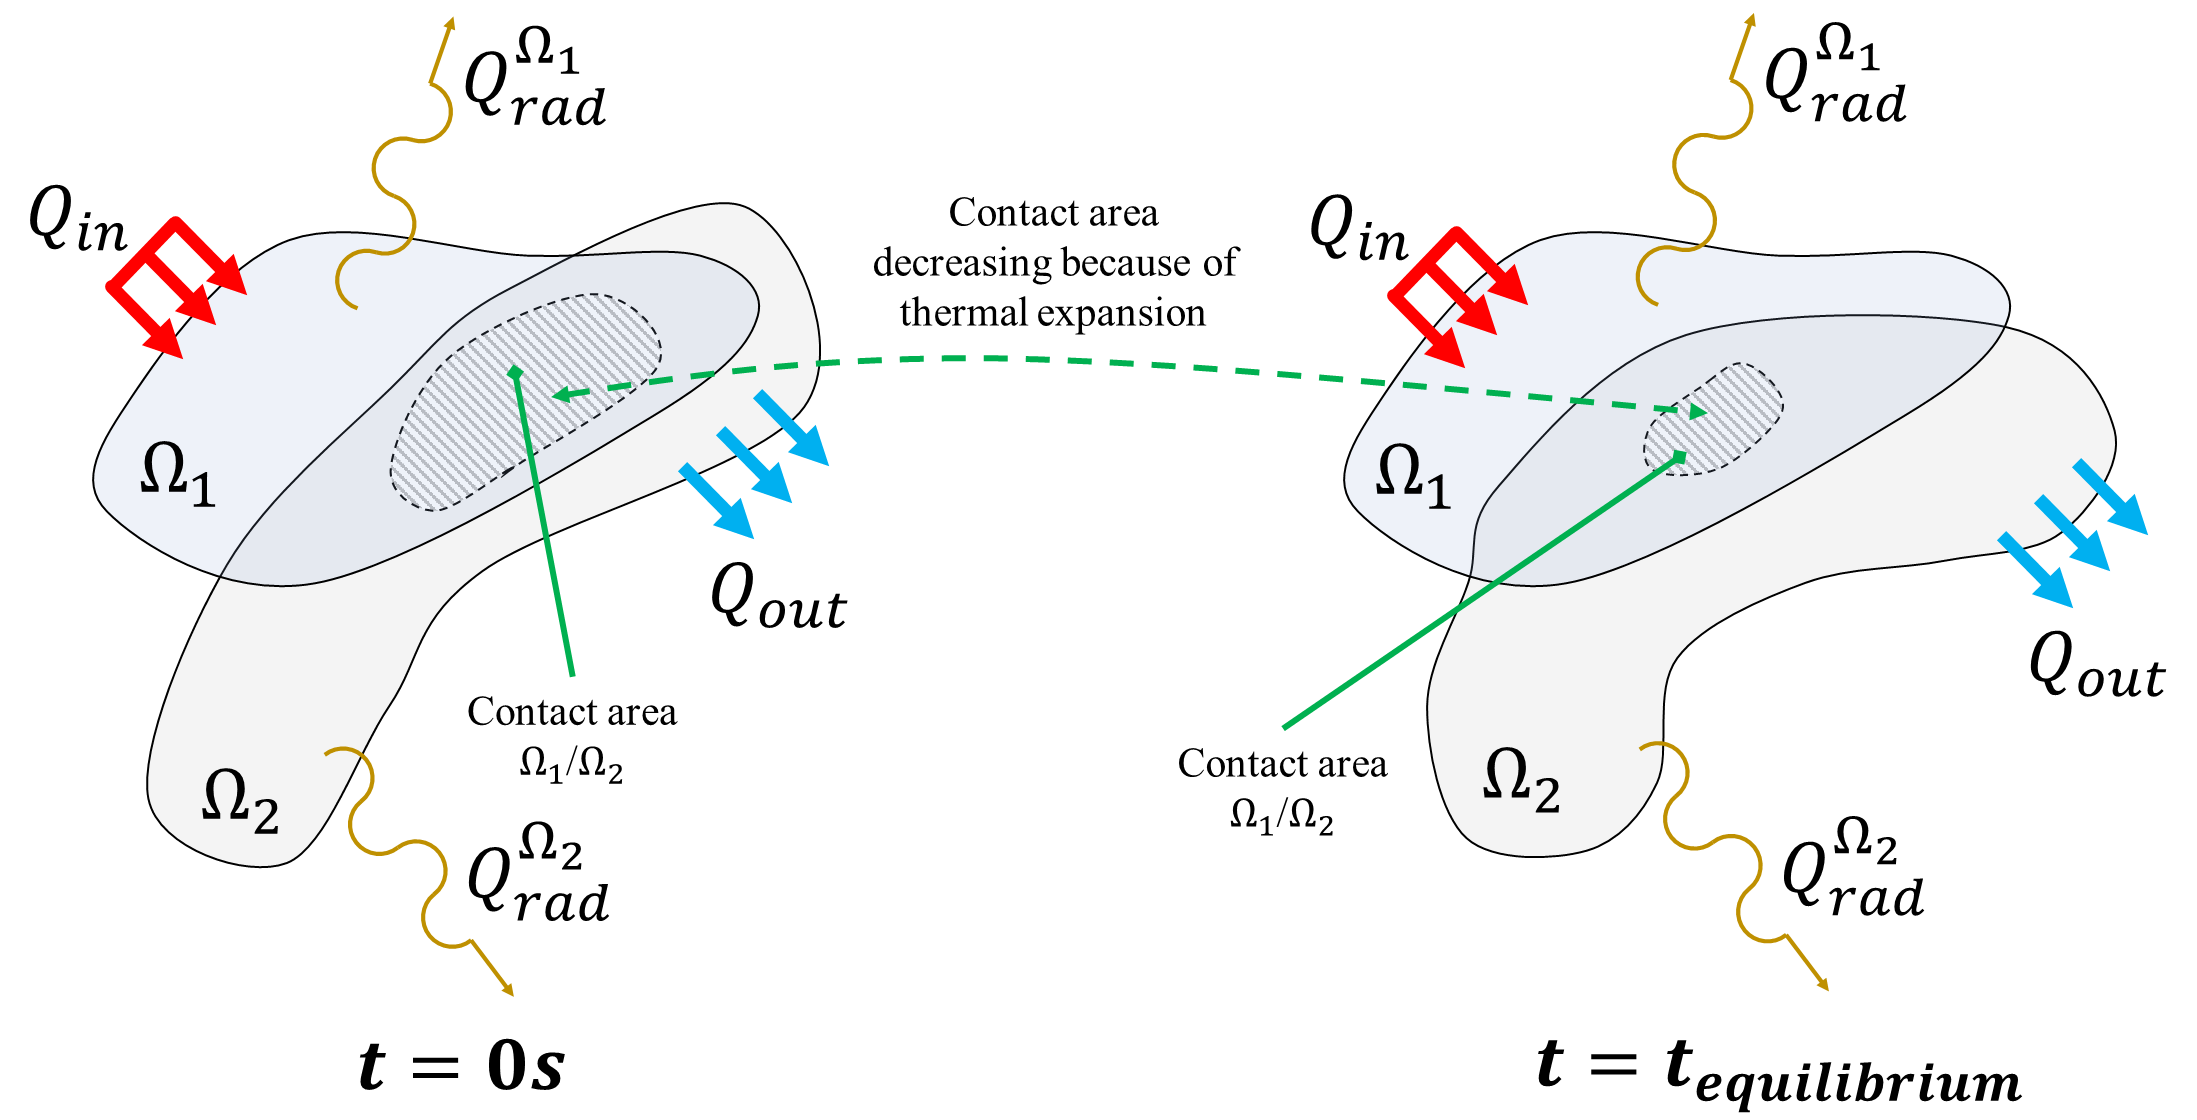
\includegraphics[width=1\textwidth]{figures/contactchangeschema.png}
    \caption{\it Contact area reduction phenomenom.}
\end{figure}
\\
\normalsize{\indent In steady-state, the input heat load $Q_{in}$ is constant. What happens is the decrease of contact area between the two domain $\Omega_1$ and $\Omega_2$ limiting the heat transfer from $\Omega_1$ to $\Omega_2$. The evacuated power $Q_{out}$ is thus lower. Because of energy conservation, the heat radiated by $\Omega_1$ is higher, increasing its temperature while the temperature of $\Omega_2$ is lower. This then leads to the first approach to coupled analysis. A first simple method was developed to "manually" update the contact geometry based on the results of the structural analysis.}
\\
\begin{figure}[!ht]
    \label{fig_5_19} 
    \centering
    
\includegraphics[width=.4\textwidth]{figures/manualCouplingMethod.png}
    \caption{\it Manual coupling method.}
\end{figure}
\\
\normalsize{\indent It is possible to test this method and perform the \acrshort{FE} analysis.}
\\
\begin{figure}[!ht]
    \label{fig_5_18}
    \centering
    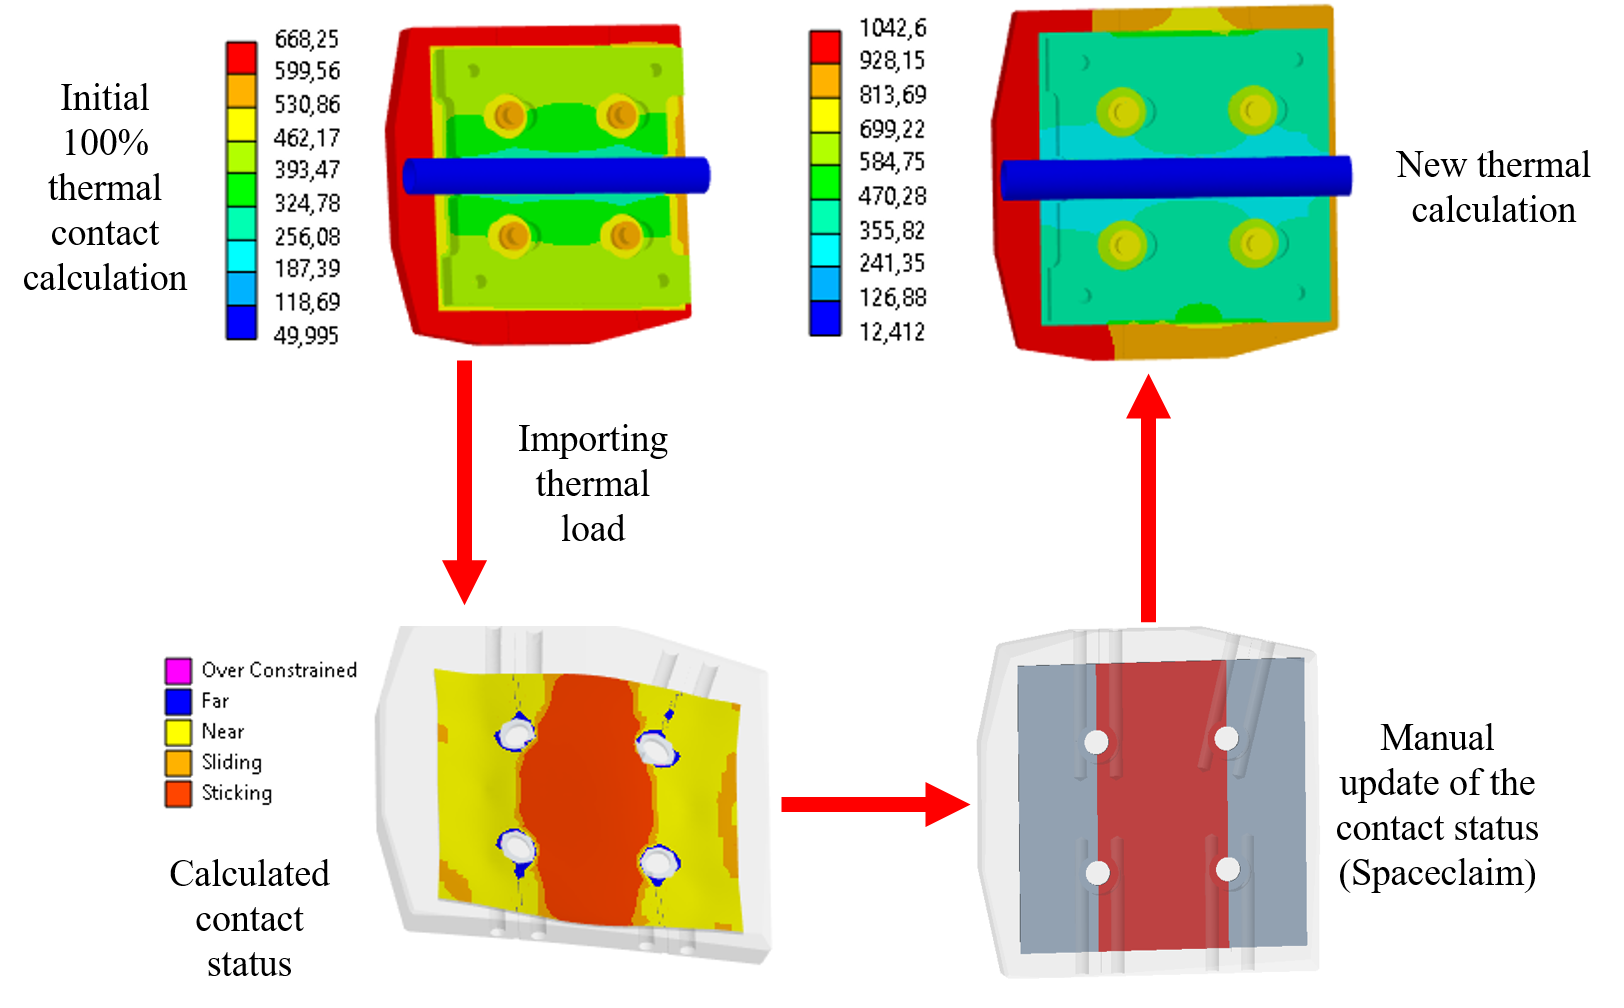
\includegraphics[width=1\textwidth]{figures/manualUpdate.png}
    \caption{\it Temperature in \unit{\si{\degree}C}. Application of the manual coupling.}
\end{figure}
\\
\normalsize{\indent In the figure above \ref{fig_5_18}, it is possible to see that the temperature field of the \acrshort{TZM} reflector tile is higher for the updated contact model. This is in accordance with the prediction by the general model \ref{fig_5_17}. The issue with the manual update is the inacuracies subsequently introduced by this manual approximation of the new contact configuration. When static structural analysis is performed on the new model, it is possible to see that the contact area tends to shrink, which is in reality not the case.}
\\
\begin{figure}[!ht]
    \label{fig_5_20}
    \centering
    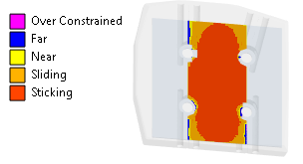
\includegraphics[width=.5\textwidth]{figures/contactShrink.png}
    \caption{\it Contact shrinking after structural recalculation.}
\end{figure}
\\
\normalsize{\indent \bfseries This conclusion leads to the logical choice of carrying out a fully coupled fields analysis to counter this complex coupled problem.}